\documentclass[12pt]{report}
\usepackage{preamble}
\graphicspath{{../img/}}

\begin{document}
\chapter{Introduction}

\section{General introduction}
Begin with a short (1–2 pages) broader introduction for a general audience: one that my mother could understand so she knows what I’ve been working on all these years.

\section{Technical introduction}
A more detailed motivation.

\subsection{Toy model: Hard spheres}

As a soft matter system:
\begin{itemize}
\item Crystallisation in hard spheres: optimal packings, Kepler conjecture in 3d
\item Similar phase diagram of real systems
\item Starting point for more complex systems
\item What is not understood? Dynamics and structure at very high densities, optimal packings in higher dimensions (computer science)
\end{itemize}

\begin{SCfigure}
  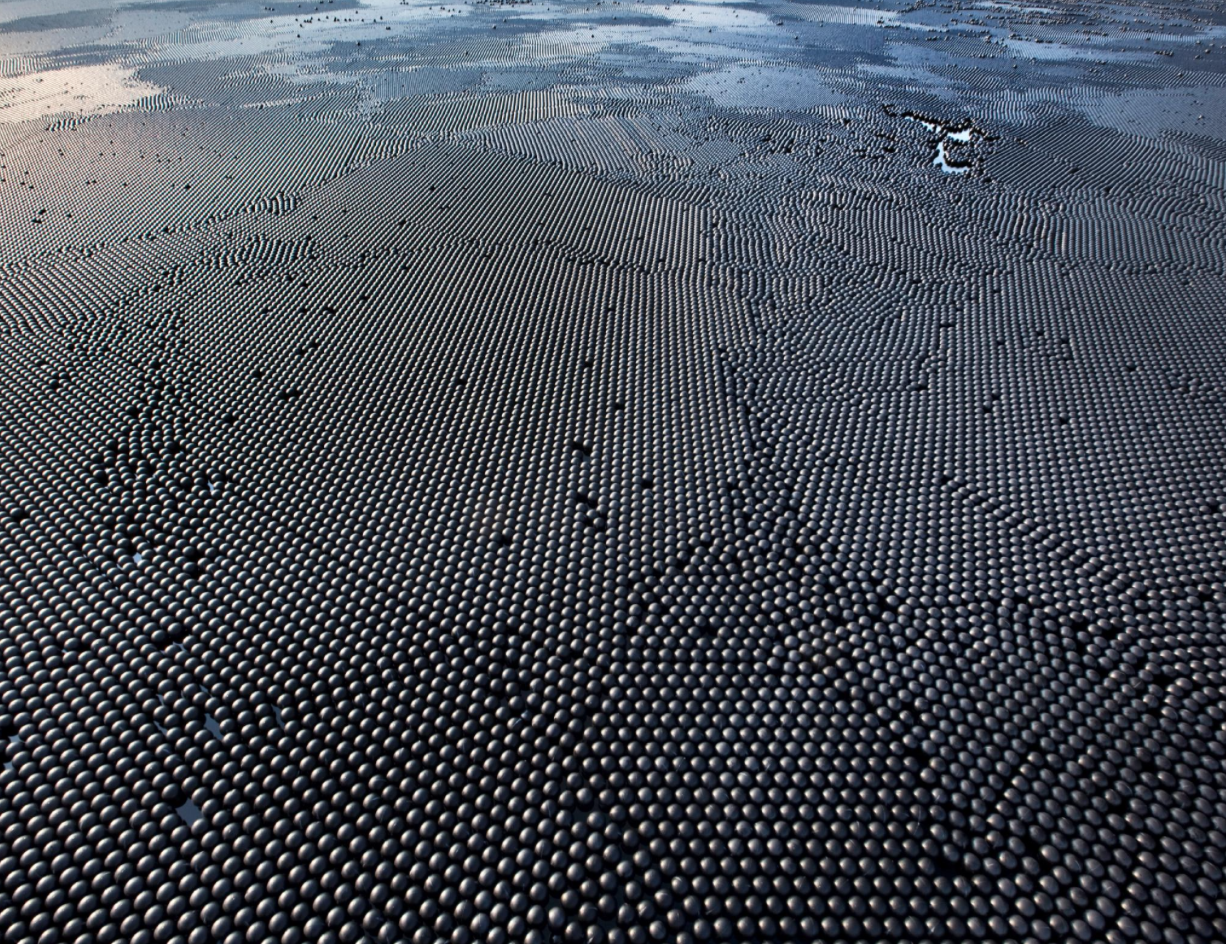
\includegraphics[width=\linewidth]{shade-balls}
  \caption{
    Shade balls covering the Los Angeles reservoir to prevent water evaporation.
    These balls spontaneously form long-range hexagonal ordering, reminiscent of crystallisation in atomic systems.
    As macroscopic objects these balls interact primarily as hard spheres.
    Image by Gerd Ludwig, \emph{National Geographic}.}
  \label{fig:shade-balls}
\end{SCfigure}

Hard spheres will spontaneously crystallise due to entropic interactions\marginfootnote{Expand on this. Why is this surprising?}[-9cm].
A similar effect is seen in balls floating on water as in e.g.\ peas in a saucepan or shade balls covering a reservoir.
The hard interactions between the balls causes\marginfootnote{In my desperate desire to use everyday examples I am cheating somewhat: while the balls certainly interact as hard spheres close to contact, I suspect there are in fact effective attractions at mid-range due to \emph{hydrodynamic} interactions at the water surface. When cooking peas in a saucepan one sees that peas will group together hexagonally even when very few of them float on the surface, i.e.\ at low densities. In contrast, hard disks should only do this at high densities.}[-8cm] 
them to `crystallise'\marginfootnote{I am cheating again, though in a smaller way this time. Strictly speaking, floating balls are two dimensionsal as they are confined to the water surface. In two dimensions it is not possible to form a crystal in the sense of long-range \emph{translational} order\cite{Mermin}, however it is possible to form a `crystal' in a less formal way of long-range \emph{orientational} order.}[-1cm] at high densities as seen in Figure \ref{fig:shade-balls}.

\end{document}
